\chapter{Application of methods}
\label{ch:applications}
In the following part of the thesis is described how to apply discussed methods to our problem. It is necessary to make several adjustments and also combine some of these methods to ensure reliable detections.

\section{Detection pipeline}
Detection is divided into three parts. All three parts are discussed in the next three subsections. The detection pipeline is visualized in Figure \ref{fig:flowchart}. 

\hspace{5px}
\begin{figure}[H]
\centering
\includegraphics[scale=0.06]{fig/flowchart.pdf}
\caption[Program pipeline]{Visualization of detection pipeline.}
\label{fig:flowchart}
\end{figure}

It can be seen that the symbolic map has two types of inputs. The main advantage of this approach is that it extends the lidar detection range. As discussed in the previous section, the used lidar has a low vertical resolution of only 16 layers. Thus the bricks are often visible in only one layer of a lidar scan. If we use only one scan, there is a high probability of false-positive measurements. On the one hand, we can decrease the occurrence of false positives by adding other lidar layers into the detection process. But on the other hand, two layers are available only from a distance smaller than $6$m, and that decreases the detection range. Therefore we exploited both approaches. One layer line segmentation for generating the candidates with low confidence and multilayer pile detector providing high-quality estimates. 

It is essential to obtain positions in the map frame, but for grasping, it is also necessary to introduce an algorithm that can give real-time feedback to the robot frame to align itself with the brick pile. When the robot is too close to the pile, it is impossible to get feedback from lidar because the bricks can be occluded, or they can be closer than the minimal lidar range. Therefore the robot needs a camera servoing for fine alignment during the brick pickup.

\section{Line segmentation}
For line segmentation, the IEPF algorithm is used, which is very similar to the one described in Algorithm \ref{alg:segmentation}. Only the final merging of parallel segments is omitted because it can connect two bricks into one. After retrieving the segments, filtering based on the segment size is done. It is possible to assign the color to the segment because each brick type has a unique size. For this reason, a new constant $max\_err$ must be defined, which thresholds out detections of incorrect size. An example of lidar measurement with extracted and filtered lines is in Figure \ref{fig:segments}. 

Algorithm performance is influenced by the correct setup of constants $C$ and $S$ (clustering and splitting distance). If we choose C too high, the algorithm could join two bricks into one segment. As described in Figure \ref{fig:piledef}, the distance between two bricks of the same color is $0.1$m. Therefore the clustering distance must always be less than $0.1$m. If the clustering distance is too low, one brick can be unintentionally divided into many segments, and without merging at the end, these segments are useless. It is necessary to bear in mind that the lidar precision, as shown in Table \ref{tab:lidar} is $\pm0.03$m, so any clustering with a distance of similar magnitude would be highly affected by sensor noise. The found segments are transformed into the map frame and passed to the symbolic map as low confidence detections. The segments are further passed to the pile detector, which can filter out false-positive detections.

\hspace{8mm}

\begin{figure}[H]
\centering
\includegraphics[scale=0.43]{fig/segments}
\caption[Line segmentation visualization]{Visualization of line segmentation. In the figure, it is evident that the bricks are well detected. This detection is done approximately from a distance of $3$m. There is one false positive detection visible behind the brick piles on a tree. The squares in the grid has $1\si{m}^2$.}
\label{fig:segments}
\end{figure}


\section{Pile detection}
\label{sec:pile_detector}
The pile detector uses one of the simplest versions of the EM algorithm. As a model for the pile is applied 2D multivariate Gaussian distribution with variance fixed to one. Although this model is not an accurate description of the detection probability, it has other advantages already discussed in previous chapters. It is easy to work with, and it converges to the global optimum very well. Only the mean value is optimized, and it should converge into the center of the pile. The stopping criterion for the algorithm is solely the number of iterations. The robot is a realtime system, and there are strict demands for meeting a deadline. 

There are further requirements for a hypothesis to be declared as a pile after the optimization is done. We look around the proposed center in a one-meter radius, and we inspect all bricks found in this area. All the following conditions must be fulfilled for segments in a pile:
\begin{enumerate}[label=(\alph*)]
\item There are at least two unique heights ($z$ positions).
\item There are at least two unique places ($(x,y)$ positions).
\item The difference between maximal and minimal height is smaller than the pile height.
\item The center of the pile is inside the arena.
\end{enumerate}
When these conditions are met, the hypothesis is declared as the pile and pushed into the symbolic map with high confidence. When at least one of these conditions is violated, then all the segments in this hypothesis are deleted, and the algorithm runs again until there are no more segments within the hypothesis radius. The condition (b) does not apply to the orange and blue pile because they have a different structure than the others. The whole procedure is shown in Algorithm \ref{alg:pile_detection}. The conditions listed above are validated in the method \textbf{is\_pile}.
\begin{algorithm}[]
 \KwData{segments}
 \KwResult{pile\_position}
\While{True}{
	pile\_position = fit\_em(segments)\;
	pile\_segments = segments\_in\_pile(pile\_position, segments)\;
	\If{pile\_segments.size() $< 2$}{
		return None\;	
	}
	\eIf{is\_pile(pile\_segments)}{
		return pile\_position\;
	}{
		segments.delete(pile\_segments)\;
	}
} 
 \caption{Algorithm to obtain pile centers.}
 \label{alg:pile_detection}
\end{algorithm}

\begin{figure}[H]
\centering
\includegraphics[scale=0.3]{fig/em_algo.png}
\caption[Em Algorithm in pile detector]{Several steps of the EM algorithm for the red pile. Colored lines are the visualized segments the same as in Figure \ref{fig:segments}. Red dots show subsequent positions of the mean value of multivariate Gaussian. Although there are many false positives, especially at the bottom of the picture, the pile model ensures that the algorithm converges to the correct place.}
\label{fig:em}
\end{figure}


\section{Pattern fitting}
As shown in Figure \ref{fig:flowchart}, the last step of the detection pipeline is pattern fitting. It is also visible that there are two types of input into this last step. Each input is used for a different type of pattern fitting. In the previous two sections, it was described how to generate candidates with different levels of confidence. This section describes how these candidates can be used for generating actual positions and how information about the spatial distribution of bricks can be exploited for the detection. The exact position of each pile and even each brick is visible in Figure \ref{fig:piledef}. The pattern in which the bricks are stacked has three degrees of freedom - position $(x, y)$ and rotation $\phi$. The goal of the pattern fitting is to find the values of these parameters in the map frame.

\subsection{Brick fitting}
The first type of fitting uses detected 3D positions of individual bricks obtained in a pile detector. The pattern defines the position of each brick, which can be detected by the lidar sensor. The next step is to generate a hypothesis that aligns this pattern with the measured positions of bricks. This step utilizes the RANSAC algorithm. Firstly we draw two different bricks from the detected set of bricks. Secondly, the correspondences are used to find the transformation - two correspondences are enough to generate the hypothesis (rotation matrix $\bm{R}$ and translation vector $\vec{t}$). The brick types (colors) and brick $z$ positions are used as the correspondences. Also, we know that the distance between corresponding pairs should match. Otherwise, it would be incorrect correspondence. Lastly, we measure the cost of the hypothesis. When the bricks are stacked into the pattern with reasonable precision, it is possible to fit the pile with average brick error down to $\pm 3$cm. After such an observation, we set the inlier distance $d_{inlier}$ to $5$cm. The algorithm is stopped after a certain number of iterations. The result is passed only if all detected bricks are inliers.

\subsubsection{Hypothesis ambiguity}
We cannot properly test the hypothesis when there are not enough bricks found. In addition, we can see the pile from behind, which renders two different patterns to match. For this reason, at least five detected red bricks are required to start the brick fitting. As shown in Figure \ref{fig:ambiguity}, even with four detected red bricks, the hypothesis can be easily fitted incorrectly. All conditions which can start fitting the hypothesis from front view are listed below:
\begin{enumerate}[label=(\alph*)]
\item 5 red bricks detected.
\item 3 green bricks detected.
\item 4 bricks of at least two colors detected.
\end{enumerate}
For the view from behind, only the condition (c) is sufficient.
\begin{figure}[H]
\centering
\includegraphics[scale=0.3]{fig/ambiguous.png}
\caption[Hypothesis ambiguity]{Two possible hypothesis which can be generated by four red bricks in their intersection are visualized in the black rectangles. This is a top view of detection from the front, so it is not visible that all red bricks are in two layers.}
\label{fig:ambiguity}
\end{figure}

\subsection{Cluster fitting}
The second type of fitting polls the clusters from the symbolic map and utilizes the confidence of clusters and their spatial distribution. For the RANSAC algorithm, a hypothesis using only four clusters would be too sparse to fit reliably. Because of this reason, the cluster fitting is done by the EM algorithm. As in pile detection, multivariate Gaussian distribution is used to represent the pile, but this time, the model takes into account relationships between positions of the piles. We define the probability model as follows:
\begin{equation}
P(\vec{x}_m) = \mathcal{N}_m(\vec{x}_m; \vec{\mu} + k_m\vec{v}; \bm{\Sigma_m}),
\label{eq:prob}
\end{equation}
where $m$ is pile (color) index, and $M$ is an absolute number of colors, $\vec{x}_m$ is a measurement of color $m$, $\vec{\mu}$ is mean value of the whole model, $\bm{\Sigma_m}$ is a covariance matrix, $k_m$ is scalar multiplier unique for each pile and $\vec{v}$ is defined as:
\begin{equation}
\vec{v} = \begin{bmatrix}
\cos \phi \\
\sin \phi
\end{bmatrix},
\end{equation}
where $\phi$ is the rotation of the model. This definition of the model ensures that all piles (Gaussians) are in line with a distance defined by multiplier $k$. How such a model could look like is visualized in Figure \ref{fig:mnd}.

\begin{figure}[H]
	\centering
	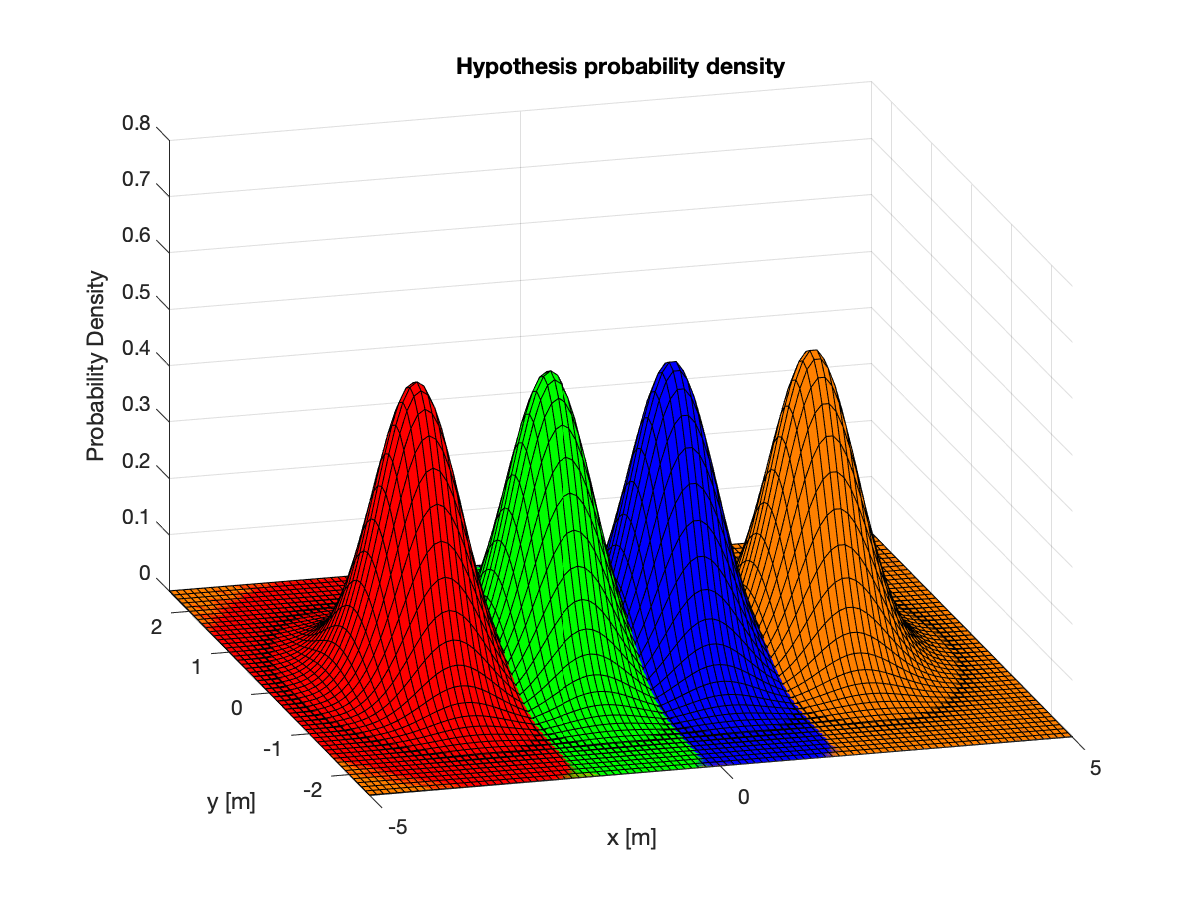
\includegraphics[scale=0.55]{fig/model_mnd.eps}
	\caption[Model of piles]{Example of a probability density function, which can be described as model \ref{eq:prob}. This particular model was created using $\vec{k}_{pile}$ from the Table \ref{tab:constants}, $\mu = [0, 0]$, $\phi$ = 0 and $\bm{\Sigma} = 0.3\bm{E}$, where $\bm{E}$ is identity matrix of size $2$.}
	\label{fig:mnd}
\end{figure}

 Now we want to obtain the position and rotation of such a model based on real measurements. There is a closed-form solution for maximizing both terms, which can be found using the maximum likelihood estimate. For mean value, the derivation is very similar to multivariate Gaussian:
\begin{align}
\frac{\partial \log\mathcal{L} }{\partial \vec{\mu}_m} &=  \bm{\Sigma}^{-1}_m \sum_{n = 1}^{N_m} (\vec{x}_{m_n} - \vec{\mu} - k_m \vec{v}), \\
\vec{\mu_m} &= \sum_{n = 1}^{N_m} \frac{\vec{x}_{m_n} - k_m \vec{v}}{N_m}.
\end{align}
Further, it is necessary to derive MLE for rotation $\phi$, which is hidden inside vector $\vec{v}$. For simplicity the matrix equation is now split into one part for each of two dimensions:
\begin{align}
\frac{\partial \log\mathcal{L}_x }{\partial \phi_m} &= \frac{1}{\sigma^2_x} \sum_{n=1}^{N_m} (x_{m_n, x} - \mu_x - k_{m, x} \cos \phi) \left( -k_{m,x} \sin \phi\right),  \\
\frac{\partial \log\mathcal{L}_y }{\partial \phi_m} &= \frac{1}{\sigma^2_y} \sum_{n=1}^{N_m} (x_{m_n, y} - \mu_y - k_{m, y} \sin \phi) k_{m,y} \cos \phi.
\end{align}
Likelihood derivative is now set equal to zero to find the extremes for each dimension:
\begin{align}
\cos \phi_m &= \frac{1}{k_{m, x}N_m} \sum_{n = 1}^{N_m} \left(  x_{m_n, x} - \mu_x \right)  , \\ 
\sin \phi_m &=  \frac{1}{k_{m, y}N_m} \sum_{n = 1}^{N_m} \left(  x_{m_n, y} - \mu_y \right)  .
\end{align}
Now it is possible to divide one equation by the other, use the basic relationship of trigonometric functions, and derive the final expression for maximizing the rotation $\phi$:
\begin{align}
\phi_m &= \arctan \left( \frac{\dfrac{\sum_{n = 1}^{N_m} \left( x_{m_n, y} - \mu_y \right)}{k_{m, y}N_m} }{ \dfrac{\sum_{n = 1}^{N_m} \left( x_{m_n, x} - \mu_x \right)}{k_{m, x}N_m} }\right).
\end{align}
Although the expression can be further simplified, in this form, it is easier to weight each data sample by the expectation $\gamma$. Also, it is necessary to consider the contribution of each color to the pile model. This can be done in two ways. One possibility is to set an equal contribution to each data sample. In our case, this could lead to bias towards the most detected color (usually red). Therefore we set equal contributions to all colors instead of the samples. The final form used in the maximization step looks as follows:
\begin{align}
\vec{\mu} =& \sum_{m=1}^M \dfrac{1}{M}\sum_{n = 1}^{N_m}  \vec{\gamma}_{m_n} \left( \vec{x}_{m_n} - k_m \vec{v} \right) , \\
\phi = \arctan & \left( \dfrac{\sum_{m=1}^{M} \dfrac{\sum_{n = 1}^{N_m} \gamma_{m_n, y}(x_{m_n, y} - \mu_y)}{k_{m, y} } }{\sum_{m=1}^{M} \dfrac{\sum_{n = 1}^{N_m} \gamma_{m_n, x} (x_{m_n, x} - \mu_x) }{k_{m, x}} }\right).
\end{align}
The method is demonstrated in Figure \ref{fig:em_pattern}. The expectation is calculated simply by evaluating the probability of sample $P(\vec{x}_m)$ as in equation \ref{eq:prob}. Results can be further improved when the confidence of the sample is used as the prior probability.

\begin{figure}[H]
	\centering
	\begin{subfigure}{0.49\textwidth}
		\centering
		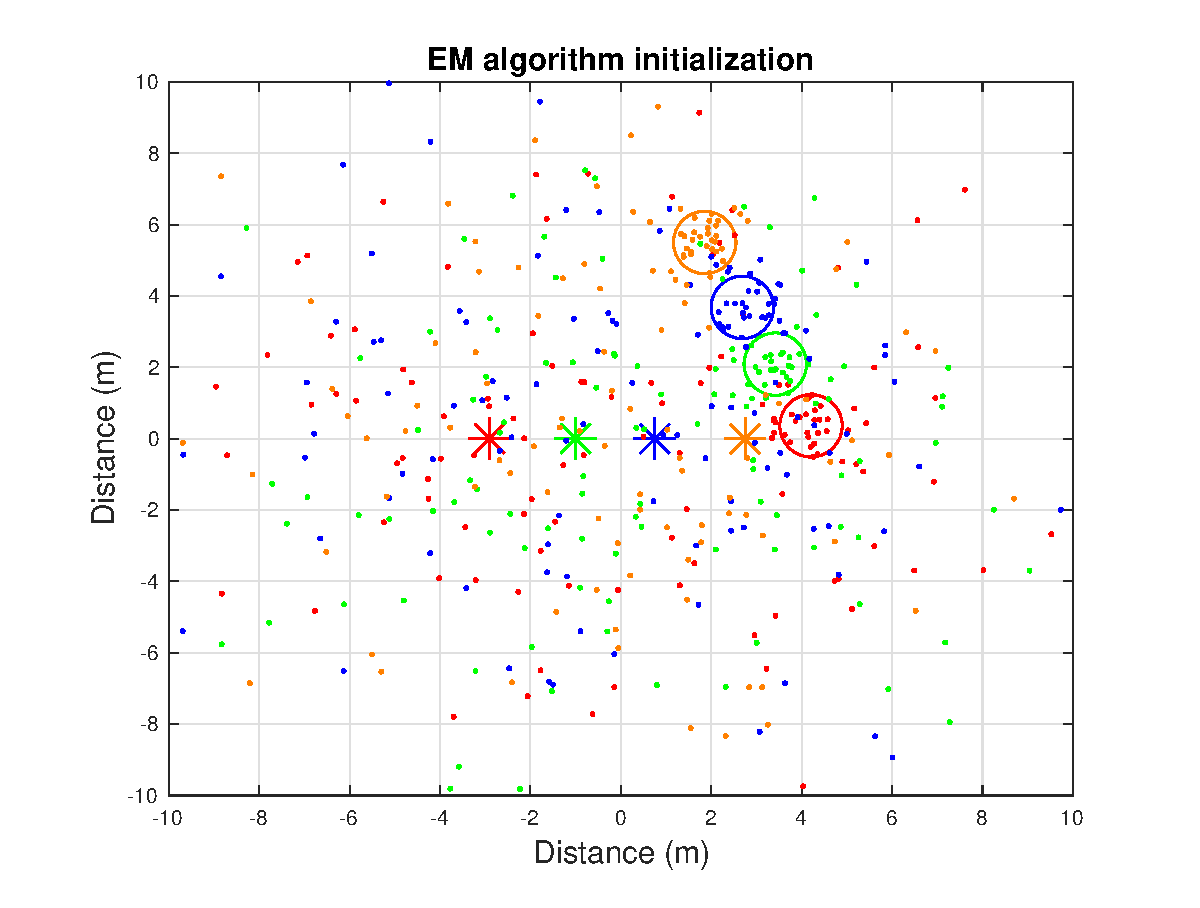
\includegraphics[scale=0.43]{fig/em_init.eps}
	\end{subfigure}
	\begin{subfigure}{.49\textwidth}
		\centering
		\includegraphics[scale=0.43]{fig/em_result.eps}

	\end{subfigure}
	
	\caption[EM pattern fitting]{In the pictures, the pattern fitting using the EM algorithm is visualized. On the left there is algorithm initialized with parameters $\vec{x}=(0, 0)$ and $\phi=0$. Stars mark the algorithm estimate. Points are generated by sampling multivariate Gaussian distribution. The model was sampled with parameters $\vec{x}=(3, 3)$ and $\phi=2$ to create the desired pattern of points. Positions of sampled piles are marked as circles. At the end of the procedure, all parameters are found correctly.}
	\label{fig:em_pattern}
\end{figure}

\subsubsection{Convergence}
The unimodality of the model's likelihood was disrupted by adding the rotation parameter to Gaussians. Possible local optimum is shown in Figure \ref{fig:em_local}. Now there are no guarantees that the algorithm converges into the global optimum. That is a common issue of the EM algorithm when dealing with more complex problems. Many solutions to this issue were proposed. Very advantageous is that local optima are usually significantly worse in terms of likelihood than the global optimum. 

One way to avoid local optima is the deterministic annealing, which influences how the expectation is used in the maximization step \cite{ueda1998}. Another way how to escape local optimum is to apply perturbations to parameters of the model. In our case, it could be, for example, rotating the model by $180\degree$. A different approach would be a population-based em algorithm with multiple initializations or informed initialization. The latter is easily applicable in our case because the confidences of clusters could be used in the expectation step. 

Because we have the formulas for gradient, it is also possible to use an arbitrary gradient ascend method instead of an MLE to maximize the likelihood of the model. The advantage of using the MLE for maximization step is that the algorithm converges very fast, and the computation is usually much faster than the computation of any gradient method.

\begin{figure}[H]
	\centering
	\begin{subfigure}{0.49\textwidth}
		\centering
		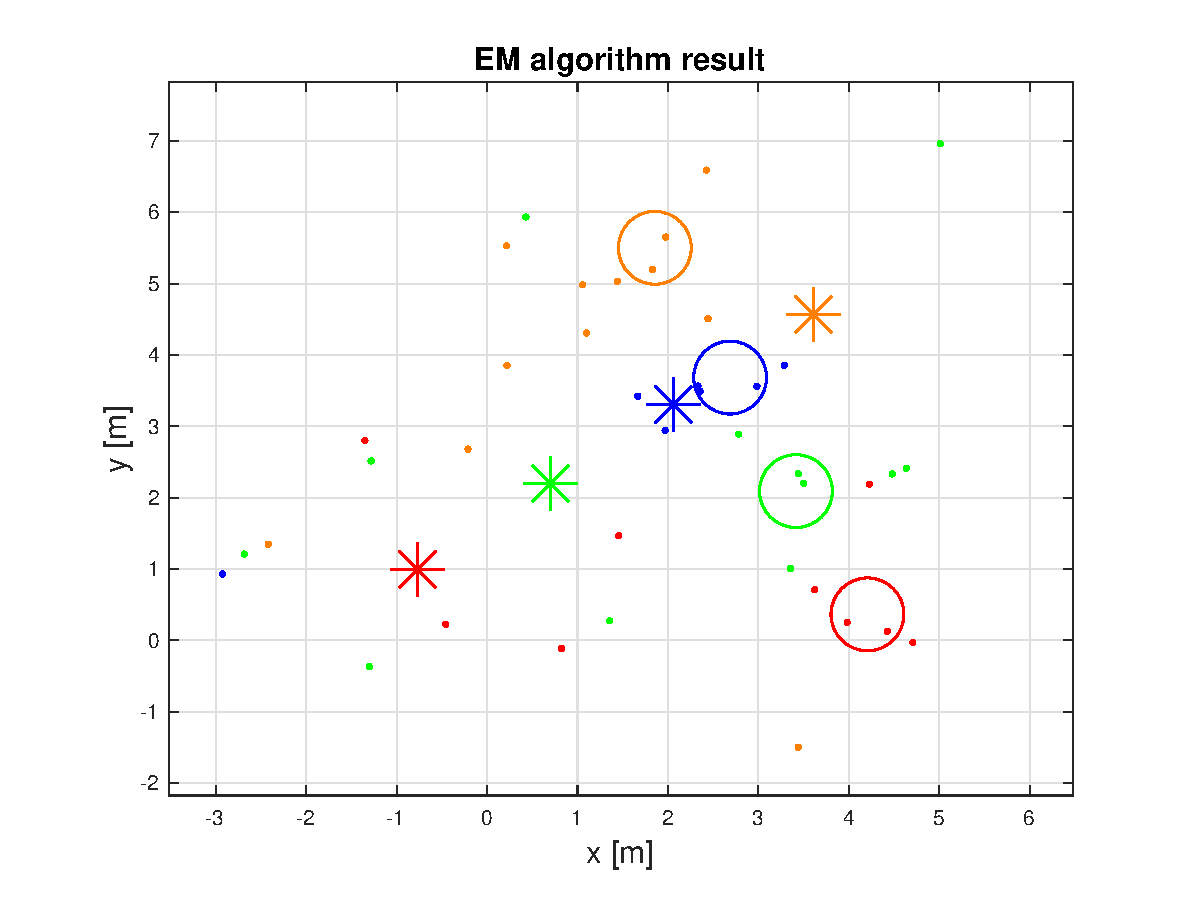
\includegraphics[scale=0.43]{fig/em_local.eps}
	\end{subfigure}
	\begin{subfigure}{.49\textwidth}
		\centering
		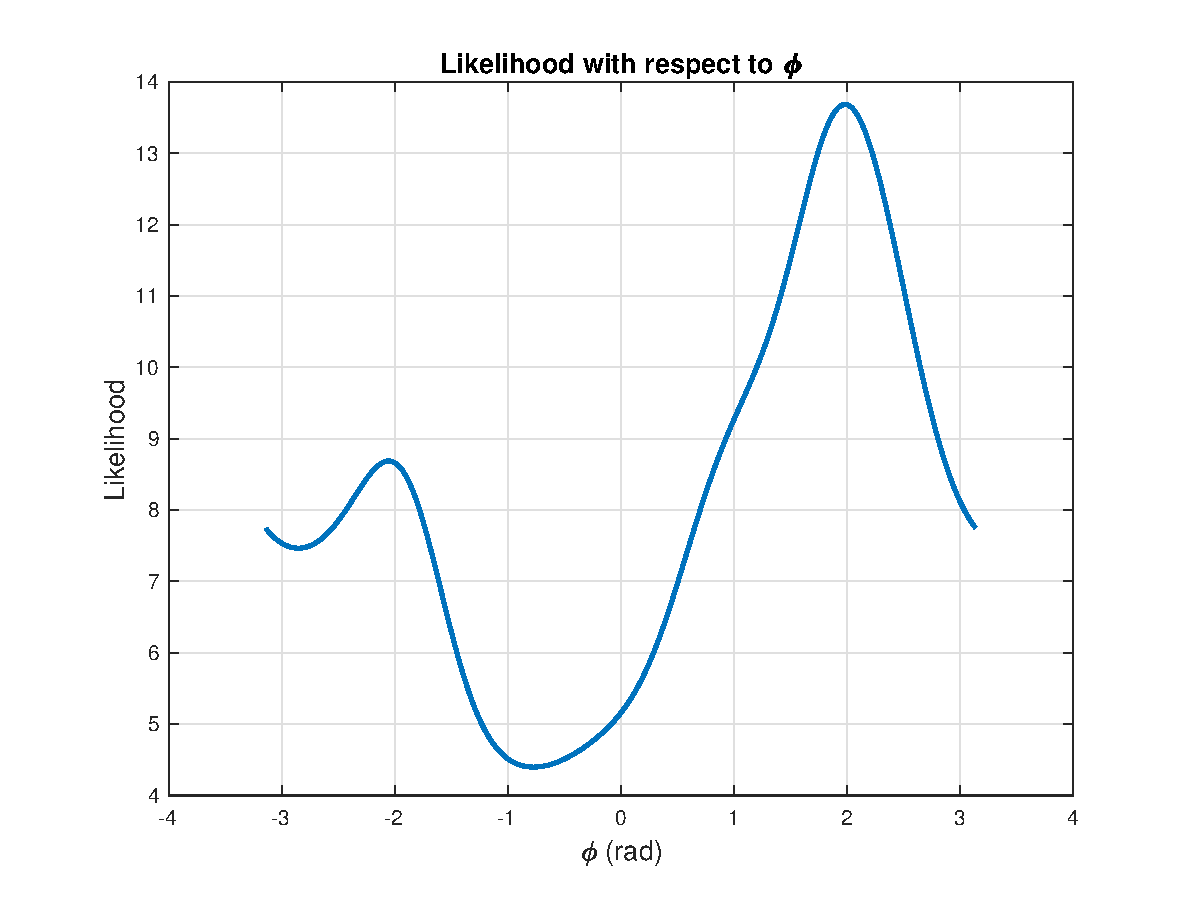
\includegraphics[scale=0.43]{fig/em_local_chart.eps}
		
	\end{subfigure}
	
	\caption[EM local optima]{When there are not enough samples, the EM algorithm is more susceptible to getting stuck in local optima, as shown on the left. The right picture shows how different rotations of the model with fixed mean influences the likelihood, and it also shows that there is a local maximum.  The likelihood is maximal when $\phi = 2$, which is the optimal rotation of the model.}
	\label{fig:em_local}
\end{figure}

\section{Arena exploration}
It is vital to emphasize on proper arena exploration. If all the interest points are not found, the robot can not proceed in completing the challenge. Except for the initial brick position, it is necessary to find also the destination where the bricks should be placed. This place is marked by the checker pattern in Figure \ref{fig:checker}. The only sensor which can detect the destination pattern is the camera. The big advantage is that the camera is mounted onto the arm so that it can be raised into height and turn around. As can be seen in Figure \ref{fig:detection_range}, the most limiting factor of the detection range is currently the UGV destination-pattern search.

\begin{figure}[H]
	\centering
	\includegraphics[scale=0.38]{fig/detection_range.png}
	\caption[Detection ranges]{In the picture, we see the range of each type of detection. Fitting the complete hypothesis with the RANSAC method (green) requires a high number of detected segments in piles, so the range is low - around $3$m. For detection of the pile (blue), just a few detected segments are required, so the detection range longer - around $5$m. The camera can obtain candidates for checker pattern (red) from the maximal distance of $8$m, which is the limit distance for exploration. From an even bigger distance, candidates for bricks (yellow) using the lidar sensor can be generated. The upper boundary can be even higher, but we set it manually to $15$m to reduce the number of false-positive detections.}
	\label{fig:detection_range}
\end{figure}

The waypoints of exploration movement should be generated so that circles cover the area of the whole arena with an $8$m radius. Generated waypoints in the arena are visualized in Figure \ref{fig:map_annot}. On each waypoint, the robot must stop, raise the arm, and look around with the camera. There are several reasons why camera detection cannot be done while moving. First of all, the arm can not be raised to the highest possible position while the robot is moving. Otherwise, it could get stuck or damaged. In addition, the motion blur of the camera would reduce the detection range even further. During camera detection, the robot must stay still, but the lidar detections can be done while moving. That can improve the detection range and speed because the robot can do measurement from many more different places. 

Whole map exploration is described in Algorithm \ref{alg:exploration}. The waypoints are ordered prior to this algorithm. How to order them is beyond the scope of this thesis. In the algorithm, it is visible that the method \textbf{start\_lidar\_detection} is non-blocking service, which just turns on the detector, whereas the method \textbf{do\_camera\_detection} is blocking service, which waits until the arm looks around with a camera and finishes the detection. This method is also the most time-consuming part of the loop.

\begin{figure}[H]
	\centering
	\includegraphics[scale=0.25]{fig/map_annotation.png}
	\caption[Generated waypoints]{Purple waypoints are places where the robot should stop and look around. Green circles are camera ranges from the corresponding place. In this figure, the waypoints are generated so that there is no unexplored area. That is usually not necessary since the objects of interest have non-negligible size. It is thus possible to further reduce the number of waypoints.}
	\label{fig:map_annot}
\end{figure}

\begin{algorithm}[H]
	\KwData{waypoints}
	done = False\;
	\While{not done}{
		waypoint = waypoints.pop()\;
		start\_lidar\_detection()\;
		go\_to(waypoint)\;
		stop\_lidar\_detection()\;
		raise\_arm()\;
		do\_camera\_detection()\;
		fold\_arm()\;
		\If{has\_all\_objects() or waypoints.empty()}{
			done = True\;	
		}
	}
	\If{not has\_all\_objects()}{
		go\_to(get\_strongest\_candidate())\;
	}
	\caption{Algorithm to explore whole map.}
	\label{alg:exploration}
\end{algorithm}

\section{Stacked bricks detection}
It is evident that when the bricks are stacked close to each other without any significant gap, it is impossible to distinguish which bricks the lidar detects. This issue was already addressed in previous chapters. It is desirable to know what color a particular lidar point has. That is done by the camera to lidar registration. Since we know the relative position of the camera to lidar and the intrinsic camera matrix, it is not a problem to assign a color to each point. The colors are further utilized during the clustering. We can now split clusters not only using the spatial data, but the splitting can be based on the color difference of the subsequent points. 

Modified clustering is visible in algorithm \ref{alg:clustering}. Input points must be from a single layer of pointcloud and ordered by yaw. Constant $C$ is clustering distance, $T$ is color clustering distance, and $min\_size$ is minimal cluster size - this has a big influence on the range of brick candidate generation. Note that the color distance is computed from the whole cluster mean to a new point. When the new point is added, the color of the cluster should be recalculated. This is important to reduce camera noise influence on the final form of clusters. When this running-mean technique is used, the clusters are split only in sharp color transitions. 

How the pointcloud coloring and final detection looks like is shown in Figure  \ref{fig:colors}. Since the robot stacked all of these bricks, their relative position should be known. Whole stacking is a predefined sequence of movements, and thus we can add each placed brick into the list of stacked bricks with its relative position to place where stacking started. These known positions can be used to generate hypothesis which can be fitted by the RANSAC algorithm in the same way as during the pattern fitting. 

When we use colors for the segmentation, it is crucial to choose the right color space. During the experiments, it was much easier to distinguish between green and blue color in LAB color space than in HSV color space. The LAB is more computationally intensive, but it is preferred color space for segmentation \cite{wang2014}. The robot is not capable of carrying orange bricks, so it was not necessary to segment the orange color, which is problematic because it can be easily confused with red color. This part of detection is not discussed any further because it was more important to localize the initial position of UGV bricks. Furthermore, placing more than one load of bricks was not achievable in the given timeframe.

\begin{algorithm}[H]
	\KwData{points}
	\KwResult{clusters}
	initialize constants C, T, min\_size \;
	cluster = [], 	clusters = []\;
	\ForEach{pt in points}{
		\eIf{cluster.empty()}{
			cluster.push\_back(pt)\;
		}{
			\eIf{distance(pt, cluster[end]) $<$ C and color\_distance(pt, cluster) $<$ T}{
				cluster.push\_back(pt)\;
			}{
				\If{cluster.size() $>$ min\_size}{
					clusters.push\_back(cluster)\;
				}
				cluster.clear()\;
			}
		}
	}
	\caption{Spatial and color clustering.}
	\label{alg:clustering}
\end{algorithm}

\begin{figure}[H]
	
	\begin{subfigure}{0.49\textwidth}
		\centering
		\includegraphics[scale=0.19]{fig/colors_camera}
	\end{subfigure}
	\begin{subfigure}{0.49\textwidth}
		\centering
		\includegraphics[scale=0.18]{fig/colors_lidar}
	\end{subfigure}
	
	\caption[Colored pointcloud detections]{Detection of bricks using color-based clustering. On the left: Image from a camera pointing at the built wall. Black dots are points captured by the lidar sensor. On the right: Final detection in map frame. All of the bricks are correctly detected, even though they are poorly painted, and the environment is very challenging.}
	\label{fig:colors}
\end{figure}

\newpage
